% THIS IS SIGPROC-SP.TEX - VERSION 3.1
% WORKS WITH V3.2SP OF ACM_PROC_ARTICLE-SP.CLS
% APRIL 2009
%
% It is an example file showing how to use the 'acm_proc_article-sp.cls' V3.2SP
% LaTeX2e document class file for Conference Proceedings submissions.
% ----------------------------------------------------------------------------------------------------------------
% This .tex file (and associated .cls V3.2SP) *DOES NOT* produce:
%       1) The Permission Statement
%       2) The Conference (location) Info information
%       3) The Copyright Line with ACM data
%       4) Page numbering
% ---------------------------------------------------------------------------------------------------------------
% It is an example which *does* use the .bib file (from which the .bbl file
% is produced).
% REMEMBER HOWEVER: After having produced the .bbl file,
% and prior to final submission,
% you need to 'insert'  your .bbl file into your source .tex file so as to provide
% ONE 'self-contained' source file.
%
% Questions regarding SIGS should be sent to
% Adrienne Griscti ---> griscti@acm.org
%
% Questions/suggestions regarding the guidelines, .tex and .cls files, etc. to
% Gerald Murray ---> murray@hq.acm.org
%
% For tracking purposes - this is V3.1SP - APRIL 2009

\documentclass{acm_proc_article-sp}

\usepackage[UTF8]{ctex}
\usepackage{supertabular}
\usepackage{booktabs}
\usepackage{multirow}
\usepackage{xcolor}


\DeclareRobustCommand{\ttfamily}{\fontfamily{lmtt}\selectfont}
\DeclareRobustCommand\sectt[1]{{\fontsize{13}{12}\bfseries\ttfamily#1}}

\newcommand{\TODO}[1]{\textcolor{red}{\textbf{To do:#1}}}
\begin{document}

\title{\textsf{\zihao{-2} 数据仓库与数据挖掘第三次大作业实验报告}}
% \titlenote{(Does NOT produce the permission block, copyright information nor page numbering). For use with ACM\_PROC\_ARTICLE-SP.CLS. Supported by ACM.}}
% \subtitle{[Extended Abstract]
% \titlenote{A full version of this paper is available as
% \textit{Author's Guide to Preparing ACM SIG Proceedings Using
% \LaTeX$2_\epsilon$\ and BibTeX} at
% \texttt{www.acm.org/eaddress.htm}}}
%
% You need the command \numberofauthors to handle the 'placement
% and alignment' of the authors beneath the title.
%
% For aesthetic reasons, we recommend 'three authors at a time'
% i.e. three 'name/affiliation blocks' be placed beneath the title.
%
% NOTE: You are NOT restricted in how many 'rows' of
% "name/affiliations" may appear. We just ask that you restrict
% the number of 'columns' to three.
%
% Because of the available 'opening page real-estate'
% we ask you to refrain from putting more than six authors
% (two rows with three columns) beneath the article title.
% More than six makes the first-page appear very cluttered indeed.
%
% Use the \alignauthor commands to handle the names
% and affiliations for an 'aesthetic maximum' of six authors.
% Add names, affiliations, addresses for
% the seventh etc. author(s) as the argument for the
% \additionalauthors command.
% These 'additional authors' will be output/set for you
% without further effort on your part as the last section in
% the body of your article BEFORE References or any Appendices.

\numberofauthors{4} %  in this sample file, there are a *total*
% of EIGHT authors. SIX appear on the 'first-page' (for formatting
% reasons) and the remaining two appear in the \additionalauthors section.
%
\author{
% You can go ahead and credit any number of authors here,
% e.g. one 'row of three' or two rows (consisting of one row of three
% and a second row of one, two or three).
%
% The command \alignauthor (no curly braces needed) should
% precede each author name, affiliation/snail-mail address and
% e-mail address. Additionally, tag each line of
% affiliation/address with \affaddr, and tag the
% e-mail address with \email.
%
% 1st. author
\alignauthor
\textsf{\large 平~国~楼}\\
       % \affaddr{软件学院}\\
       \affaddr{学号:2019312652}\\
       % \affaddr{Wallamaloo, New Zealand}\\
       \email{pgl19@mails.tsing hua.edu.cn}
% 2nd. author
\alignauthor
\textsf{\large 徐~荣~琛}\\
       % \affaddr{软件学院}\\
       \affaddr{学号:2019214518}\\
       % \affaddr{Dublin, Ohio 43017-6221}\\
       \email{xrc19@mails.tsing hua.edu.cn}
% 3rd. author
\alignauthor
\textsf{\large 杨~~~柳}\\
       % \affaddr{软件学院}\\
       \affaddr{学号:2018214187}\\
       % \affaddr{Hekla, Iceland}\\
       \email{yang18@mails.tsing hua.edu.cn}
\and  % use '\and' if you need 'another row' of author names
% 4th. author
\alignauthor 
\textsf{\large 甘~伟~冲}\\
       % \affaddr{软件学院}\\
       \affaddr{学号:2019312661}\\
       % \affaddr{P.O. Box 5000}\\
       \email{ganwc19@mails.ts inghua.edu.cn}
}
% There's nothing stopping you putting the seventh, eighth, etc.
% author on the opening page (as the 'third row') but we ask,
% for aesthetic reasons that you place these 'additional authors'
% in the \additional authors block, viz.
% \additionalauthors{Additional authors: John Smith (The Th{\o}rv{\"a}ld Group,
% email: {\texttt{jsmith@affiliation.org}}) and Julius P.~Kumquat
% (The Kumquat Consortium, email: {\texttt{jpkumquat@consortium.net}}).}
% \date{30 July 1999}
% Just remember to make sure that the TOTAL number of authors
% is the number that will appear on the first page PLUS the
% number that will appear in the \additionalauthors section.

\maketitle
% \begin{abstract}
% This paper provides a sample of a \LaTeX\ document which conforms to
% the formatting guidelines for ACM SIG Proceedings.
% It complements the document \textit{Author's Guide to Preparing
% ACM SIG Proceedings Using \LaTeX$2_\epsilon$\ and Bib\TeX}. This
% source file has been written with the intention of being
% compiled under \LaTeX$2_\epsilon$\ and BibTeX.

% The developers have tried to include every imaginable sort
% of ``bells and whistles", such as a subtitle, footnotes on
% title, subtitle and authors, as well as in the text, and
% every optional component (e.g. Acknowledgments, Additional
% Authors, Appendices), not to mention examples of
% equations, theorems, tables and figures.

% To make best use of this sample document, run it through \LaTeX\
% and BibTeX, and compare this source code with the printed
% output produced by the dvi file.
% \end{abstract}

% % A category with the (minimum) three required fields
% \category{H.4}{Information Systems Applications}{Miscellaneous}
% %A category including the fourth, optional field follows...
% \category{D.2.8}{Software Engineering}{Metrics}[complexity measures, performance measures]

% \terms{Delphi theory}

% \keywords{ACM proceedings, \LaTeX, text tagging} % NOT required for Proceedings

\section{\textsf{\zihao{-4}银行精准营销解决方案}}
该部分主要解决的任务是根据提供的银行营销数据,构建合适的分类模型,预测客户是否会购买该银行的产品。

% 首先对数据进行特征正则化、特征独热化和数据集降维与拆分等数据预处理,然后采用K折交叉验证,并对MLP、
% SVM、DT、LR、PLR等分类器进行训练评估,其中PLR为自己实现的分类器。最后根据Accuracy、F1和P这3个
% 评价指标,得到了样本均衡化和未均衡化的实验结果。

\subsection{\textsf{\zihao{-4}数据预处理}}
数据预处理过程一共包括特征正则化处理、基于pd.get\_dummies()特征独热化处理、数据集降维与拆分三个步骤。

\subsubsection{\textsl{\zihao{5}特征正则化处理}}
% 特征正则化处理按以下步骤执行:

\newcommand{\normalizing}[1]{$\text{#1} = \frac{\text{#1}}{\max(\text{#1})-\min(\text{#1})}$}

\begin{enumerate}\setlength\itemsep{0mm}
       \item 删除ID特征
       \item \normalizing{age}
       \item \normalizing{balance}
       \item \normalizing{duration}
       \item \normalizing{campaign}
       \item \normalizing{pdays}
       \item \normalizing{previous}
       \item $\text{day} =\text{day}+30\times int(\text{mouth})$ \\
       \normalizing{day}
       \item 删除month列
\end{enumerate}
% \begin{supertabular}{ll}
%        (1)& 删除ID特征\\
%        (2)& \normalizing{age}\\
%        (3)& \normalizing{balance}\\
%        (4)& \normalizing{duration}\\
%        (5)& \normalizing{campaign}\\
%        (6)& \normalizing{pdays}\\
%        (7)& \normalizing{previous}\\
%        (8)& $\text{day} =\text{day}+30\times int(\text{mouth})$\\
%        & \normalizing{day}\\
%        (9)& 删除month列\\
% \end{supertabular}
\subsubsection{\textsl{\zihao{5}基于}pd.get\_dummies()\textsl{\zihao{5}特征独热化处理}}
% 基于pd.get\_dummies()特征独热化处理按以下步骤执行:

\begin{enumerate}\setlength\itemsep{0mm} 
       \item  Job转化为12位的独热码
       \item  marital转化为3位的独热码
       \item  education转化为4位的独热码
       \item  housing转化为2位的独热码
       \item  loan转化为2位的独热码
       \item  contact转化为3位的独热码
       \item  poutcome转化为4位的独热码(可以调整)
       \item  default转化为1位的独热码
\end{enumerate}
% \begin{supertabular}{ll}
%        (1)&	Job转化为12位的独热码\\
%        (2)&	marital转化为3位的独热码\\
%        (3)&	education转化为4位的独热码\\
%        (4)&	housing转化为2位的独热码\\
%        (5)&	loan转化为2位的独热码\\
%        (6)&	contact转化为3位的独热码\\
%        (7)&	poutcome转化为4位的独热码(可以调整)\\
%        (8)&	default转化为1位的独热码\\
% \end{supertabular}

\subsubsection{\textsl{数据集降维与拆分}}
% 数据集降维与拆分按以下步骤执行:
\begin{enumerate}\setlength\itemsep{0mm} 
       \item  拆分label与data;
       \item  Data降维,使用方法包括PCA、FastICA、LDA。PCA、FastICA降维后的维数为20,LDA降维后的维数为2;
       \item  合并label与data;
       \item  提取正负样本,其中正样本数2961,负样本数22356。
\end{enumerate}
% \begin{supertabular}{ll}
%        (1)&	拆分label与data。\\
%        (2)&	Data降维,使用方法包括PCA、FastICA、\\
%        & LDA。PCA、FastICA 降维后的维数为20, \\
%        &LDA降维后的维数为2。\\
%        (3)&	合并label与data。\\
%        (4)&	提取正负样本,其中正样本数2961,负样本\\
%        &数22356。\\
% \end{supertabular}

\subsection{\textsf{\zihao{-4}不同方法的交叉验证实验}}
\begin{enumerate}\setlength\itemsep{0mm} 
       \item  设置交叉验证折数为8;
       \item  设置算法,包括MLP、SVM、DT、LR、PLR,其中PLR为自写;
       \item  设置评价指标,包括Accuracy,F1,P (查准率);
       \item  删除少量样本,使正负样本总数都为折数的倍数。其中删除正样本1个,负样本4个,剩余正样本2960个,负样本22352个;
       \item  以下二选一,包括均衡与不进行均衡的情况:
       \begin{itemize}\setlength\itemsep{0mm} 
              \item 提取每次交叉验证的训练集与测试集并对正负样本进行均衡化,使正样本数目等于负样本数目,均衡方法为正样本
              首先进行多次倍数级联,少于单倍个数的进行随机补足;
              \item 不进行均衡化;
       \end{itemize}
       \item  进行训练和测试,得到评价指标。
\end{enumerate}
% \begin{supertabular}{ll}
%        (1)&   设置交叉验证折数为8。\\
%        (2)&	设置算法,包括MLP、SVM、DT、LR、\\
%        & PLR,其中PLR为自写。\\
%        (3)&	删除少量样本,使正负样本总数都为折数的\\
%        & 倍数。其中删除正样本1个,负样本4个,\\
%        & 剩余正样本2960个,负样本22352个。\\
%        (4)&	提取正负样本,其中正样本数2961,负样本\\
%        &数22356。\\
%        (5)&	以下二选一,包括均衡与不进行均衡的情况:\\
%        & $\bullet$ 提取每次交叉验证的训练集与测试集并对\\
%        & 正负样本进行均衡化,使正样本数目等于负\\
%        & 样本数目,均衡方法为正样本首先进行多次\\
%        & 倍数级联,少于单倍个数的进行随机补足。\\
%        & $\bullet$ 不进行均衡化。\\
%        (6)&	进行训练和测试,得到评价指标\\
% \end{supertabular}

\subsection{\textsf{\zihao{-4}实验结果}}
进行均衡的实验结果如表(\ref{JHSY})所示。未进行均衡的结果如表(\ref{WJHSY})所示。

\begin{table}[!ht]
\centering
\small
\caption{均衡实验结果}
\setlength{\tabcolsep}{1.4mm}{
\begin{tabular}{@{}c@{\hskip 0mm}c|ccccc@{}}
\toprule
\multicolumn{2}{c|}{}                    & SVM                               & DT                               & MLP                              & LR                               & PLR \\ \midrule
\multirow{3}{*}{原特征}             &ACC  &0.809                              &\textcolor{red}{0.700}            &\textcolor{red}{\textbf{0.816}}   &\textcolor{red}{0.814}            &0.725\\
                                   &F1   &0.805                              &\textcolor{red}{0.608}            &\textbf{0.814}                    &\textcolor{red}{0.810}            &0.780\\
                                   &P    &0.673                              &\textcolor{red}{\textbf{0.879}}   &\textcolor{red}{0.822}            &0.826                             &0.651\\ \midrule
\multirow{3}{*}{PCA$_{20}$}        &ACC  &0.673                              &0.598                             &\textbf{0.688}                    &0.678                             &0.591\\
                                   &F1   &0.655                              &0.409                             &0.656                             &\textbf{0.674}                    &0.612\\
                                   &P    &0.692                              &\textbf{0.772}                    &0.730                             &0.681                             &0.581\\ \midrule
\multirow{3}{*}{IDA$_2$}           &ACC  &\textcolor{red}{0.812}             &0.642                             &\textbf{0.813}                    &0.799                             &\textcolor{red}{0.809}\\
                                   &F1   &\textcolor{red}{0.816}             &0.506                             &\textcolor{red}{0.820}            &0.787                             &\textcolor{red}{\textbf{0.825}}\\
                                   &P    &0.798                              &0.815                             &0.790                             &\textcolor{red}{\textbf{0.836}}   &\textcolor{red}{0.761}\\ \midrule
\multirow{3}{*}{FastICA$_{20}$}    &ACC  &0.585                              &0.628                             &\textbf{0.677}                    &\textbf{0.677}                    &0.659\\
                                   &F1   &0.307                              &0.472                             &0.666                             &0.674                             &\textbf{0.687}\\
                                   &P    &\textcolor{red}{\textbf{0.931}}    &0.810                             &0.690                             &0.681                             &0.635\\ \bottomrule
\end{tabular}
}
\label{JHSY}
\end{table}

\begin{table}[!ht]
\centering
\small
\caption{未均衡实验结果}
\setlength{\tabcolsep}{1.4mm}{
\begin{tabular}{@{}c@{\hskip 0mm}c|ccccc@{}}
\toprule
\multicolumn{2}{c|}{}                    & SVM                        & DT                               & MLP                       & LR                               & PLR \\ \midrule
\multirow{3}{*}{原特征}             &ACC  &0.893                       &\textcolor{red}{0.880}            &\textcolor{red}{0.899}     &\textcolor{red}{\textbf{0.901}}   &\textcolor{red}{0.845}\\
                                   &F1   &0.285                       &\textcolor{red}{\textbf{0.498}}   &0.463                      &\textcolor{red}{0.434}            &\textcolor{red}{0.380}\\
                                   &P    &\textcolor{red}{0.647}      &\textcolor{red}{0.487}            &0.615                      &\textbf{0.651}                    &\textcolor{red}{0.457}\\ \midrule
\multirow{3}{*}{PCA$_{20}$}        &ACC  &\textbf{0.893}              &0.835                             &0.892                      &\textbf{0.893}                    &0.586\\
                                   &F1   &0.285                       &\textbf{0.304}                    &0.272                      &0.273                             &0.285\\
                                   &P    &\textcolor{red}{0.647}      &0.300                             &0.641                      &\textcolor{red}{0.668}            &0.178\\ \midrule
\multirow{3}{*}{IDA$_2$}           &ACC  &\textcolor{red}{0.900}      &0.853                             &\textcolor{red}{0.899}     &0.899                             &0.263\\
                                   &F1   &\textcolor{red}{0.463}      &0.368                             &0.429                      &0.423                             &0.030\\
                                   &P    &0.625                       &0.370                             &0.634                      &\textbf{0.635}                    &0.018\\ \midrule
\multirow{3}{*}{FastICA$_{20}$}    &ACC  &0.883                       &0.839                             &0.892                      &\textbf{0.893}                    &0.636\\
                                   &F1   &0.000                       &\textbf{0.320}                    &0.255                      &0.273                             &0.310\\
                                   &P    &0.000                       &0.316                             &\textcolor{red}{0.664}     &\textcolor{red}{0.668}            &0.199\\ \bottomrule
\end{tabular}
}
\label{WJHSY}
\end{table}
其中,加粗表示在本列(所有方法中)取得最大值,同时取得最大值时,都加粗。红色字体表示在本行(所有降维方法中),该指标取得
最大值,由于包括三个指标,所以每列至少有三个指标进行加粗。

\subsection{\textsf{\zihao{-4}评价}}

使用了交叉验证方法,设置交叉验证折数为8,由于在银行营销预测的结果通常用于产品推荐,因此为了不较少打扰无意愿购买产品的客户,
比较重视查准率,因此我们使用了查准率P指标,其次F1一定程度上反应了查准率和查全率均衡的情况,我们也使用了该指标,另外预测准
确率作为最常用的预测指标,最能反应模型的性能,所以总体上我们使用了Accuracy、F1、P三个评价指标,同时也使用了PCA、LDA、
FastICA等降维方法。

\subsubsection{\textsl{\zihao{5}均衡情况}}

针对模型:使用了MLP、SVM、DT、LR、PLR,其中PLR为自写,总体上MLP>LR>SVM>PLR>DT指标 另外,自写的回归算法PLR结果总体上
比sklearn提供的LR差。

针对数据:原特征即选择了所有特征,并进行了相应的预处理,降维方法使用了PCA、LDA、FastICA,PCA、 FastICA 降维后维数为
20, LDA降维后维数为2。原特征在MLP、DT、LR上取得了最佳结果,LDA在SVM、PLR上取得了最佳结果,因此,在所有降维方法中,
LDA方法的结果明显优于其他方法。

\subsubsection{\textsl{\zihao{5}未均衡情况}}

总体上,相对于进行了均衡的情况,ACC大幅提高,F1与P大幅下降。

针对模型:使用了MLP、SVM、DT、LR、PLR,其中PLR为自写,总体上LR>MLP>SVM>DT>PLR指标 另外,自写的回归算法PLR结果
总体上比sklearn提供的LR差的比较多。

针对数据:原特征即选择了所有特征,并进行了相应的预处理,降维方法使用了PCA、LDA、FastICA,PCA、 FastICA 降维后维数
为20,LDA降维后维数为2。原特征在MLP、DT、LR、PLR上取得了最佳结果,LDA在SVM上取得了最佳结果,因此,在所有降维方法中,
LDA方法的结果明显优于其他方法。

\section{\textsf{\zihao{-4}学生调查问卷结果分析}}

该部分主要解决的任务是:根据提供的调查问卷的回答结果,对学生进行类型划分,分析每种类型的特点,
并结合数据对学生、老师或学校提出建议。

\subsection{\textsf{\zihao{-4}实验准备}}
实验准备包括数据预处理、聚类算法和实验评价指标选择的介绍。
\subsubsection{\textit{数据预处理}}

数据预处理包括人工的特征选择和自动化的数据降维方法两个部分。其中,自动化的数据降维采用PCA技术。
人工的特征选择是基于问题语义的特征选择。尝试的一种人工的特征选择是注意到分析的核心是调查问卷,故我们将关注的重点放在调查问卷的问题
特征之中,而删去所有的其它特征。
对于预处理降维对聚类结果的影响会在后续实验环节进行评估。

% \subsubsection{\textit{特征选择}}

% \subsection{\textsf{\zihao{-4}聚类算法}}
\subsubsection{\textit{聚类算法}}

在对数据进行预处理之后,我们使用KMeans、MiniBatchKMeans以及DBSCAN聚类算法进行聚类
实验和分析,其中对KMeans算法进行了手工实现,所有的详细代码实现可参见Data.py文件。

\subsubsection{\textit{实验评价指标选择}}

因为本次实验数据中并没有对数据类型的标注,因此我们选择了轮廓系数、Calinski-Harabasz指数和
Davies-Bouldin指数等三种无标的聚类评价指标作为此次实验的评价指标,下面给出这三种指标的简要介绍。

% \subsubsection{\textit{实验评价指标选择}}
\textbf{轮廓系数}(Silhouette Coefficient)是聚类效果好坏的一种评价方式。
% 最早由Peter J. 
% Rousseeuw 在 1986 提出。
它结合内聚度和分离度两种因素。可以用来在相同原始数据的基础上用
来评价不同算法、或者算法不同运行方式对聚类结果所产生的影响。
对于数据点$i \in C_i$(数据点$i$位于聚簇$C_i$中)
$$a(i) = \frac{1}{|C_i| - 1} \sum_{j \in C_i, i \neq j} d(i, j)$$
代表数据点$i$到其相同簇内所有点的平均距离。
$$b(i) = \min_{k \neq i} \frac{1}{|C_k|} \sum_{j \in C_k} d(i, j)$$
代表数据点$i$到其不同簇内所有点的平均距离点最小值。于是数据点$i$的轮廓系数
$$s(i) = \frac{b(i) - a(i)}{\max\{a(i),b(i)\}}$$
将所有点的轮廓系数求平均,就是该聚类结果总的轮廓系数
$$\mathit{SC}=\frac{1}{|N|} \sum_{i\in N} s(i)$$

\textbf{Calinski-Harabasz指数}是%T. Calinski和J. Hara-basz于1974年提出的
一种基于同一聚类
内部平方的平均值以及不同聚类之内平方和的平均值评估聚类有效性的方法。以下的数学公式给出了其的计算式:
$$\mathit{CH} = \frac{ tr(B_k) }{ tr(W_k) } \times \frac{ N-k }{ k-1 }$$
其中,$N$是训练样本数,$k$为类别数,$B_k$为类别之间的协方差矩阵,$W_k$为类别内部数据的协方差矩阵,
$tr$用于求解矩阵的迹。

\textbf{Davies-Bouldin指数}是一种基于数据集样本数量和特征数量聚类质量度量方法。
%由David L. 
%Davies和Donald W. Bouldin于1979年提出。
$n$维样本,$C_i$是某个聚簇。 $X_j$是$C_i$中的样本。 定义$S_i$是簇内紧凑性的量度:
$$S_i = \left(\frac{1}{T_i} \sum_{j=1}^{T_i} {\left| X_j-A_i\right|^p}\right)^{1/p}$$
其中$A_i$是$C_i$的聚簇中心,$T_i$是$C_i$的样本数目,通常$p$取2代表欧几里得距离。
定义$M_{i,j}$是簇$C_i$、$C_j$间分离性的量度:
$$M_{i,j} = \left|\left|A_i-A_j\right|\right|_p = \Bigl(\displaystyle\sum_{k=1}^{n}\left|a_{k,i}-a_{k,j}\right|^p\Bigr)^{\frac 1 p}$$
其中,$a_{k,i}$代表$A_i$的第$k$个元素。定义$R_{i,j}$表示簇$i$和簇$j$间的聚簇质量度量:
$$R_{i,j} = \frac{S_i + S_j}{M_{i,j}}$$
对于某个簇$i$定义$D_i$表示簇$i$的聚簇质量:
$$D_i \equiv \max_{j \neq i} R_{i,j}$$
若一共有$N$个簇,则:
$$\mathit{DB} \equiv \frac{1}{N}\displaystyle\sum_{i=1}^N D_i$$

\subsection{\textsf{\zihao{-4}实验说明}}

\begin{table*}[!ht]
       \small
       \centering
       \caption{降维对聚类算法影响评估}
       \begin{tabular}{@{}c|c|ccc|ccc|ccc@{}}
       \toprule
                     &\multicolumn{1}{c|}{\multirow{2}{*}{维度}} & \multicolumn{3}{c|}{KMeans} & \multicolumn{3}{c|}{MiniBatchKMeans} & \multicolumn{3}{c}{DBSCAN} \\
                     &\multicolumn{1}{c|}{}                     & $K=2$   & $K=3$   & $K=4$   & $K=2$      & $K=3$      & $K=4$      & $M=150$ & $M=160$ & $M=170$ \\ \midrule
       未降维         & 33                                       & 1.0000  & 1.0000  & 1.0000  & 1.0000     & 1.0000     & 1.0000     & 1.0000  & 1.0000  & 1.0000  \\
       人为属性选择    & 28                                       & 0.9931  & 0.9903  & 0.5539  & 0.9694     & 0.9585     & 0.9050     & 0.2054  & 0.2610  & 0.1955  \\
       PCA 98\%      & 23                                       & 0.9993  & 0.9978  & 0.9993  & 0.9904     & 0.9362     & 0.9368     & 0.6811  & 0.6403  & 0.4806  \\
       PCA 95\%      & 14                                       & 1.0000  & 0.9997  & 0.9551  & 0.9978     & 0.9175     & 0.9207     & 0.4398  & 0.5761  & 0.4411  \\
       PCA 90\%      & 6                                        & 0.9993  & 0.9957  & 0.9958  & 0.9896     & 0.9661     & 0.9286     & 0.1817  & 0.2312  & 0.1732  \\ 
       PCA 80\%      & 2                                        & 0.9990  & 0.9903  & 0.9840  & 0.9955     & 0.9084     & 0.9819     & 0.1793  & 0.2277  & 0.1704  \\ 
       PCA 50\%      & 1                                        & 0.9983  & 0.9848  & 0.5889  & 0.9907     & 0.9627     & 0.6573     & 0.1793  & 0.2277  & 0.1704  \\ \bottomrule
       \end{tabular}
       \label{DIM}
\end{table*}
       
实验包括降维对聚类算法的影响、自实现KMeans与sklearn库的比较、超参数选择对聚类算法的影响三个部分。

\subsubsection{\textit{降维对聚类算法的影响}}
以未降维的数据经过聚类后结果为基准,考虑降维之后数据经过聚类后结果与基准的相似度。我们认为,一个“好”的降维,
即降维后数据仍然保持了原有的主体性质,因此与基准的相似度应当尽可能接近。我们基于Jacarrd距离定义以下的聚类
$C$基于聚类$B$相似度度量:
$$Sim(C,B) = \frac{1}{|C|}\sum_{c_i\in C}\max_{c_j\in B}d_{J}(c_i,c_j)$$
其中,Jacarrd距离:
$$d_{J}(A,B) = \frac{|A\cap B|}{|A\cup B|}$$
考虑基于语义的人为属性选择、98\%主成分PCA、95\%主成分PCA和90\%主成分PCA,分别对KMeans算法、MiniBatchKMeans
算法与DBSCAN算法基于某些最佳参数下的相似度度量。由于PCA方法可能存在一定随机性(初始随机点),对于每个情况进行若干
次的重复实验,取最大的相似度度量作为本组的相似度度量。实验结果如表(\ref{DIM})所示。

从表(\ref{DIM})可知,降维处理对KMeans、MiniBatchKMeans有较好的表现,特别是$K$值较小时(1、2时),即便PCA降维到1维
降维后结果与不降维结果的集合相似度仍然超过99\%。对于DBSCAN,降维对其结果影响较大,分析原因可能是降维使得某些原本DBSCAN不聚类的噪声点
被融入到非噪声点之中,这样导致了较大规模的结果变化。

\subsubsection{\textit{自实现KMeans与sklearn库的比较}}
在本次实验使用的聚类算法中,我们通过手动实现了KMeans算法,将其和算法库中的KMeans算法在不同的超参数下进行对比,
具体的实验结果见表(\ref{IMPL}),其中impl表示自主实现的KMeans算法,sklearn表示sklearn中的KMeans算法。

\begin{table}[!htb]
\small
\centering
\caption{自实现KMeans与标准库比较}
\begin{tabular}{@{}c|c|cccc@{}}
\toprule
                            & 来源        & 时间 & $\mathit{SC}$ & $\mathit{CH}$ & $\mathit{DBI}$ \\ \midrule
\multirow{2}{*}{$k=2$}      & impl        &1.29&0.3006&3534&1.2262\\
                            & sklearn     &0.61&0.3027&3562&1.2144\\ \midrule
\multirow{2}{*}{$k=3$}      & impl        &1.44&0.2466&2794&1.3797\\
                            & sklearn     &0.71&0.2581&3106&1.2212\\ \midrule
\multirow{2}{*}{$k=4$}      & impl        &1.49&0.1888&2319&1.8266\\
                            & sklearn     &0.71&0.2531&2791&1.2756\\ \bottomrule
\end{tabular}
\label{IMPL}
\end{table}
       
从聚类算法耗时角度看:纵向对比,无论是自主实现还是sklearn库,算法执行时间会随着聚类超参数K的增加而增加;
横向对比,sklearn库耗时比自主实现更短。

从三个评价指标来看:纵向对比,sklearn库随着K增加,轮廓系数和CH指数都是逐渐减少,而DBI逐渐增加,
根据三个指标的评估标准(轮廓系数和CH指数越大效果越好,DBI越小越好),可见当K为2时聚类效果越好。
而自主实现三个指标的结果随着参数K变化出现震荡,不过同样是在k=2时聚类效果最好,即轮廓系数和CH指数最大,
DBI最小;横向对比,k=2时,自主实现与sklearn库效果相近,且都达到最好效果。随着K增加,自主实现的轮廓
系数和CH指数都比sklearn库小,DBI更大,即效果更差。

\subsubsection{\textit{超参数选择对聚类算法的影响}}

考虑到聚类的效果和聚类算法以及算法内部中某些超参数的选择十分相关,为了探究KMeans算法、MiniBatchKMeans
算法与DBSCAN算法的最佳参数选择,设置了该比较实验。

对于KMeans算法、MiniBatchKMeans算法,枚举的聚类个数$K$可以进行不同参数的比较。对于DBSCAN算法,假设我们已知了参数MinPts
(简记$M$),可以利用k-距离曲线得到最佳的Eps的值(简记$E$,拐点位置,实验中我们通过寻找二阶导数的最值来确定具体的拐点),之后首先从一个
大范围大步长的参数比较找到最佳范围,随后逐渐缩小范围和步长,最终求得最佳参数。

超参数选择的实验结果如表(\ref{ARG})所示,其中KM、MK、DS分别是KMeans算法、MiniBatchKMeans
算法与DBSCAN算法的简写,SC、CH、DB分别代表轮廓系数、Calinski-Harabasz指数和
Davies-Bouldin指数三种评价指标(前两者越大越好,第三个越小越好)。限于篇幅,选取的超参数是若干代表性取值。

\begin{table}[!htb]
\small
\centering
\caption{超参数选择的评估结果}
\begin{tabular}{@{}ccccc@{}}\toprule
算法     & 超参数 & $\mathit{SC}$ & $\mathit{CH}$ & $\mathit{DB}$  \\ \midrule
KM & $K=2$   & \textbf{0.3027} & \textbf{3563} & \textbf{1.214}\\
KM & $K=3$   & 0.2581 & 3106 & 1.431\\
KM & $K=4$   & 0.2532 & 2791 & 1.275\\
KM & $K=5$   & 0.2501 & 2623 & 1.318\\\midrule
MK & $K=2$   & \textbf{0.3552} & \textbf{3556} & \textbf{1.086}\\
MK & $K=3$   & 0.2488 & 2988 & 1.424\\
MK & $K=4$   & 0.2344 & 2658 & 1.330\\
MK & $K=5$   & 0.2438 & 2445 & 1.315\\\midrule  
DS & $M=150,E=3.74$    & 0.2048 & 2231 & 1.170\\
DS & $M=155,E=3.74$    & 0.1988 & 2201 & 1.172\\
DS & $M=160,E=3.74$    & \textbf{0.3549} & \textbf{3042} & \textbf{1.032}\\
DS & $M=165,E=3.74$    & 0.2917 & 2714 & 1.452\\
DS & $M=170,E=3.74$    & 0.2917 & 2714 & 1.452\\\bottomrule
\end{tabular}
\label{ARG}
\end{table}

从表(\ref{ARG})中可知,对于各个聚类算法自身而言,三个评估指标均是一致的。对于KMaens和MiniBatchKMeans,
最优的$K$值为2,对于DBSCAN而言最优的$M$和$E$分别为160和3.74。有趣的是,对于聚类算法之间的比较,三个算法均附加最优的参数时,三个评估指标的结果
恰各不一样,轮廓系数认为MiniBatchKMeans的表现最佳,Calinski-Harabasz指数认为KMeans的表现最佳,而
Davies-Bouldin指数认为DBSCAN的表现最佳。

% \textbf{KMeans超参数选择:}

% \textbf{MiniBatchKMeans超参数选择:}

% \textbf{KMeans超参数选择:}

\subsection{\textsf{\zihao{-4}算法评价与应用}}
本部分首先通过可视化展示证明聚类算法的有效性和合理性,随后将对聚类的结果进行分析并提出对于调查问卷结果的
一些建议。

\subsubsection{\textit{可视化展示}}
为了证明聚类算法的结果能够符合直观规律,分别对KMeans算法、MiniBatchKMeans算法与DBSCAN算法在最优参数
下的结果进行可视化展示。高维数据的可视化展示采用t-SNE算法实现。



图(\ref{PKM})、(\ref{PMK})、(\ref{PDS})分别是KMeans算法、MiniBatchKMeans算法以及
DBSCAN算法的聚类结果。从图中可知,以上三种方法得到的聚类结果符合直观规律。对于DBSCAN算法,由于算法本身的原因
注意到聚类结果之中有一部分数据未能够被分到任何一个聚簇之中,即图(\ref{PDS})之中的黑色样本点,这样数据共计
有1845个。

\subsubsection{\textit{分析与建议}}
实验中,当聚成2时聚类效果最好,下面根据聚成2类时的实验结果进行分析并提出建议。
聚成2类时,类a各个问题答案平均值在1.4左右,中位数1.0,类b各个问题答案平均值2.25
左右,中位数2.5,即类b问卷答案优于类a。
问卷一共对3名教师和13门课程进行了调查,下面根据属于每位老师或者课程的答案分布情况进行分析:

3个教师分布分别是[349,426],[645,799],[2154,1447]。
可见,教师1和2的满意率占比较高,教师3的满意率较低。

13门课程中,满意度较低的课程为class3,class4,class13,而这几门课基本都是教师3授课(class13为教师2和教师3一同授课)。其中class13各个问题评分都偏低。

对教师3的问卷答案情况进行分析,发现教师3课程的平均出勤率较低,为1.56,且关于课程目标和规划类的问题的得分总体偏低,例如问题Q1和Q2,因此对老师和学校提出几点建议:
\begin{enumerate}
       \item 建议该教师在开课时和学生明确课程基本信息,如课程内容,目标以及评价体系;
       \item 建议该教师通过提高课程趣味性和增加出勤检查等方式来提升课堂出勤率;
       \item 建议学校更加注重对教师教学质量的考核,依据考核结果对课程的授课教师进行科学指导或调整,从而保证课程质量。
\end{enumerate}

% The following two commands are all you need in the
% initial runs of your .tex file to
% produce the bibliography for the citations in your paper.
\bibliographystyle{abbrv}
\bibliography{sigproc}  % sigproc.bib is the name of the Bibliography in this case
% You must have a proper ".bib" file
%  and remember to run:
% latex bibtex latex latex
% to resolve all references
%
% ACM needs 'a single self-contained file'!
%
%APPENDICES are optional
%\balancecolumns
\clearpage

% \newpage

\appendix
%Appendix A
\section{\textsf{\zihao{-4}聚类算法可视化结果}}
% \subsection{KMeans\textsf{\zihao{-4}可视化结果}}
\begin{figure}[!h]
\centering
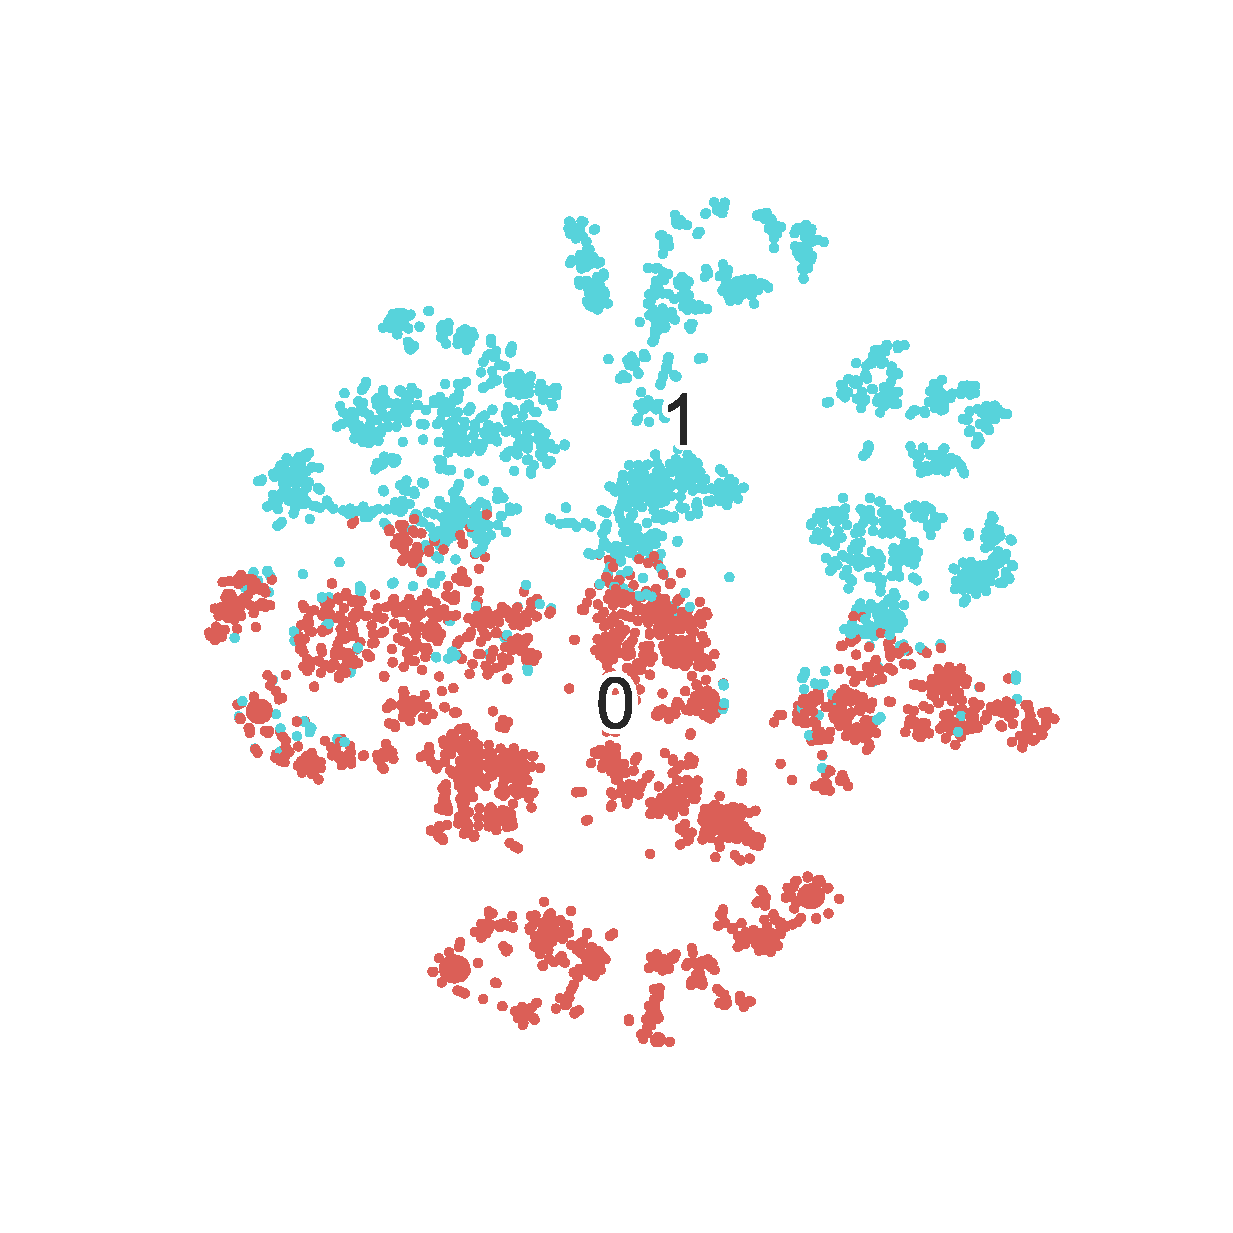
\epsfig{file=KMEANS.eps, height=3.3in, width=3.3in}
\caption{KMeans聚类结果可视化}
\label{PKM}
\end{figure}
% \subsection{MiniBatchKMeans\textsf{\zihao{-4}可视化结果}}
\begin{figure}[!h]
\centering
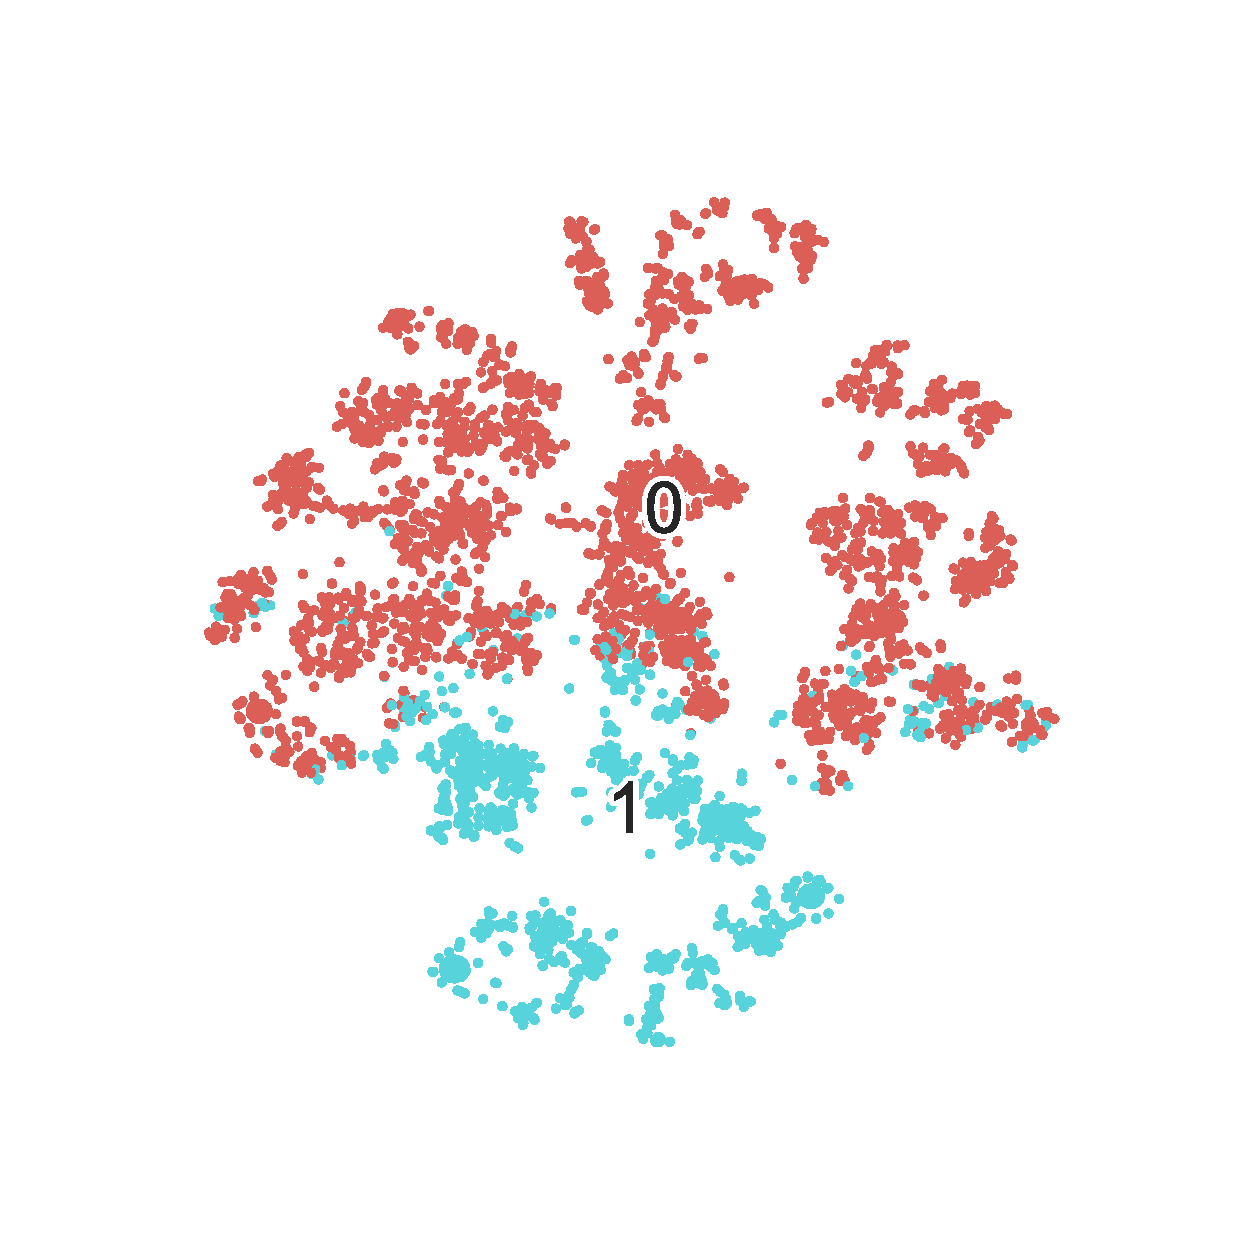
\epsfig{file=MBKM.eps, height=3.3in, width=3.3in}
\caption{MiniBatchKMeans聚类结果可视化}
\label{PMK}
\end{figure}
% \subsection{DBSCAN\textsf{\zihao{-4}可视化结果}}
\begin{figure}[!h]
\centering
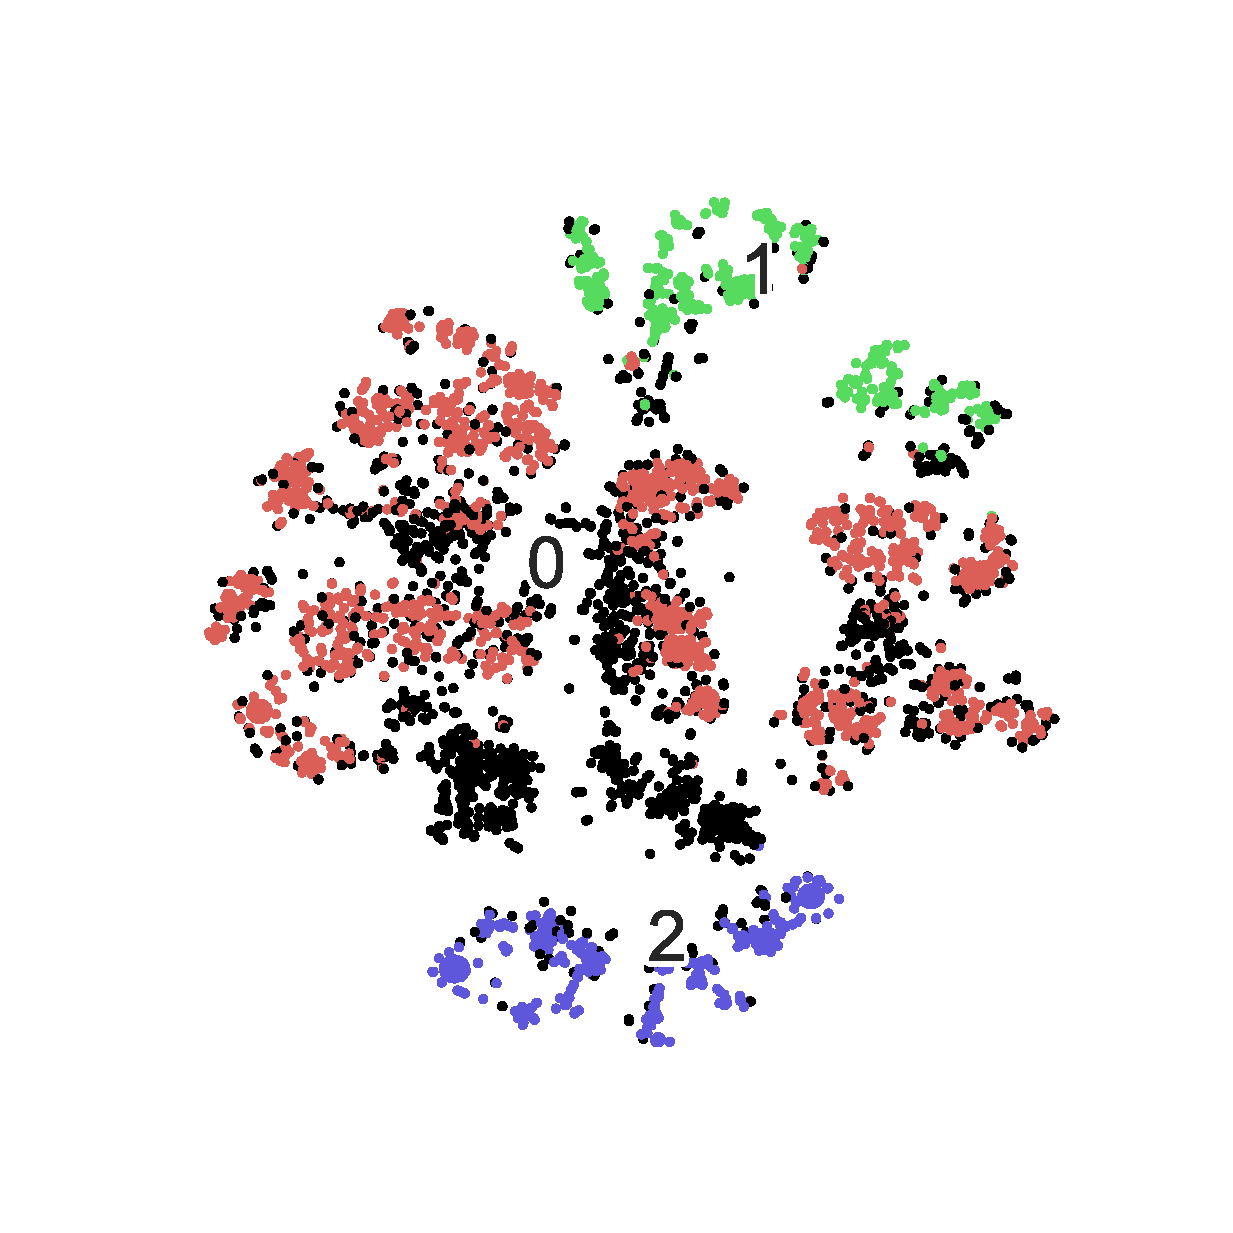
\epsfig{file=DBSCAN.eps, height=3.3in, width=3.3in}
\caption{DBSCAN聚类结果可视化}
\label{PDS}
\end{figure}
\balancecolumns
% That's all folks!
\end{document}
